\section{Chemical energetics}
\subsection{Exothermic and endothermic reactions}

An exothermic reactions transfers thermal energy to the surroundings leading to an increase in the
temperature of the surroundings. An endothermic reaction takes in thermal energy from the 
surroundings leadin gto a decrease in the temperature of the surroundings.

The transfer of energy during a reaction is caleed the enthalpy change, $\Delta H$ of the reaction.
The value is negative for exothermic reactions and positive for endothermic reactions.

Activation energy, $E_a$ is the minimum energy that colliding particles must have to react.
\begin{center}
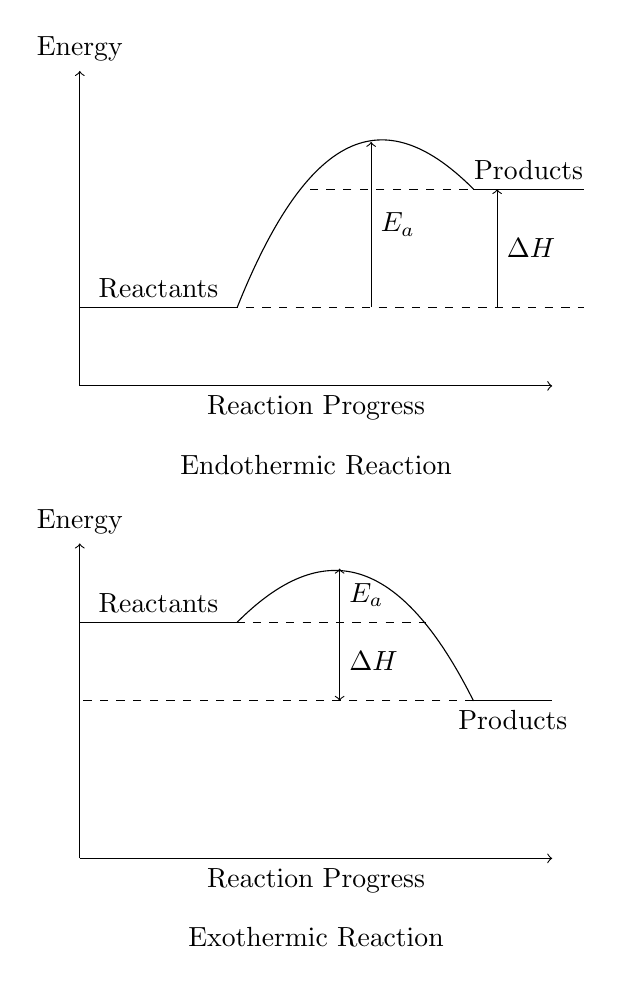
\begin{tikzpicture}

    % Axes for Endothermic Reaction
    \draw[->] (0,0) -- (6,0) node[below, midway] {Reaction Progress};
    \draw[->] (0,0) -- (0,4) node[above] {Energy};

    % Reactants for Endothermic
    \draw (0,1) -- (2,1) node[above, midway] {Reactants};
	\draw[dashed] (0, 1) -- (6.4, 1);

    % Activation energy curve for Endothermic
    \draw (2,1) .. controls (3,3.5) and (4,3.5) .. (5,2.5);

    % Products for Endothermic
    \draw (5,2.5) -- (6.4,2.5) node[above, midway] {Products};
	\draw[dashed] (6.4, 2.5) -- (2.8, 2.5);

    % Activation energy arrow for Endothermic
    \draw[->] (3.7,1) -- (3.7,3.1) node[midway,right] {$E_a$};

    % Enthalpy change arrow for Endothermic
    \draw[->] (5.3,1) -- (5.3,2.5) node[midway,right] {$\Delta H$};

    % Label Endothermic
    \node at (3,-1) {Endothermic Reaction};

    % Axes for Exothermic Reaction (below)
    \draw[->] (0,-6) -- (6,-6) node[below, midway] {Reaction Progress};
    \draw[->] (0,-6) -- (0,-2) node[above] {Energy};

    % Reactants for Exothermic
    \draw (0,-3) -- (2,-3) node[above, midway] {Reactants};

    % Activation energy curve for Exothermic
    \draw (2,-3) .. controls (3,-2) and (4,-2) .. (5,-4);

    % Products for Exothermic
    \draw (5,-4) -- (6,-4) node[midway, below] {Products};

    % Activation energy arrow for Exothermic
    \draw[->] (3.3,-3) -- (3.3,-2.32) node[midway,right] {$E_a$};
	\draw[dashed] (0.3, -3) -- (4.4, -3);

    % Enthalpy change arrow for Exothermic
    \draw[<-] (3.3,-4) -- (3.3,-3) node[midway,right] {$\Delta H$};
	\draw[dashed] (5, -4) -- (0, -4);

    % Label Exothermic
    \node at (3,-7) {Exothermic Reaction};

\end{tikzpicture}
\end{center}
Above are reaction pathway diagrams, showing the energy of a reaction as it progresses. The
energy of products is greater than that of the reactants in endothermic reactions and the opposite
is true for exothermic reactions. The differences in energy and their correspondences are labelled.

Remember that M-EXO (making is exo) and B-ENDO (breaking is endo).

Bond breaking is an endothermic process and bond making is an exothermic process. When a reaction,
overall, has bonds broken with more energy than bonds made, it is endothermic. The opposite is
also applies.

Enthalpy change can be calculated as:
\begin{center}
	enthalpy = (energy needed to break bonds) - (energy needed to
	make bonds)
\end{center}
\[\Delta H = E_b - E_f\]
where $E_b$ is the energy needed to break bonds and $E_f$ is that needed to form bonds.
